This section describes the data files for a \mf Groundwater Transport (GWT) Model.  A GWT Model is added to the simulation by including a GWT entry in the MODELS block of the simulation name file.

There a single type of spatial discretization approaches that can be used with the LNF Model: DISL.

The LNF Model is designed to permit input to be gathered, as it is needed, from many different files.  Likewise, results from the model calculations can be written to a number of output files. The LNF Model Listing File is a key file to which the LNF model output is written.  As \mf runs, information about the LNF Model is written to the LNF Model Listing File, including much of the input data (as a record of the simulation) and calculated results.  Details about the files used by each package are provided in this section on the LNF Model Instructions.

The LNF Model reads a file called the Name File, which specifies most of the files that will be used in a simulation. Several files are always required whereas other files are optional depending on the simulation. The Output Control Package receives instructions from the user to control the amount and frequency of output.  Details about the Name File and the Output Control Package are described in this section.


\subsection{Units of Length and Time}
The GWF Model formulates the groundwater flow equation without using prescribed length and time units. Any consistent units of length and time can be used when specifying the input data for a simulation. This capability gives a certain amount of freedom to the user, but care must be exercised to avoid mixing units.  The program cannot detect the use of inconsistent units.

\subsection{Steady-State Simulations}
A steady-state transport simulation is represented by a single stress period having a single time step with the storage term set to zero. Setting the number and length of stress periods and time steps is the responsibility of the Timing Module of the \mf framework.

\subsection{Volumetric Budget}
A summary of all inflow (sources) and outflow (sinks) of solute mass is called a mass budget.  \mf calculates a mass budget for the overall model as a check on the acceptability of the solution, and to provide a summary of the sources and sinks of mass to the flow system.  The solute mass budget is printed to the LNF Model Listing File for selected time steps.

\subsection{Time Stepping}


\newpage
\subsection{LNF Model Name File}
The PRT Model Name File specifies the options and packages that are active for a PRT model.  The Name File contains two blocks: OPTIONS  and PACKAGES. The length of each line must be 299 characters or less. The lines in each block can be in any order.  Files listed in the PACKAGES block must exist when the program starts. 

Comment lines are indicated when the first character in a line is one of the valid comment characters.  Commented lines can be located anywhere in the file. Any text characters can follow the comment character. Comment lines have no effect on the simulation; their purpose is to allow users to provide documentation about a particular simulation. 

\vspace{5mm}
\subsubsection{Structure of Blocks}
\lstinputlisting[style=blockdefinition]{./mf6ivar/tex/prt-nam-options.dat}
\lstinputlisting[style=blockdefinition]{./mf6ivar/tex/prt-nam-packages.dat}

\vspace{5mm}
\subsubsection{Explanation of Variables}
\begin{description}
% DO NOT MODIFY THIS FILE DIRECTLY.  IT IS CREATED BY mf6ivar.py 

\item \textbf{Block: OPTIONS}

\begin{description}
\item \texttt{list}---is name of the listing file to create for this PRT model.  If not specified, then the name of the list file will be the basename of the PRT model name file and the '.lst' extension.  For example, if the PRT name file is called ``my.model.nam'' then the list file will be called ``my.model.lst''.

\item \texttt{PRINT\_INPUT}---keyword to indicate that the list of all model stress package information will be written to the listing file immediately after it is read.

\item \texttt{PRINT\_FLOWS}---keyword to indicate that the list of all model package flow rates will be printed to the listing file for every stress period time step in which ``BUDGET PRINT'' is specified in Output Control.  If there is no Output Control option and ``PRINT\_FLOWS'' is specified, then flow rates are printed for the last time step of each stress period.

\item \texttt{SAVE\_FLOWS}---keyword to indicate that all model package flow terms will be written to the file specified with ``BUDGET FILEOUT'' in Output Control.

\end{description}
\item \textbf{Block: PACKAGES}

\begin{description}
\item \texttt{ftype}---is the file type, which must be one of the following character values shown in table~\ref{table:ftype-prt}. Ftype may be entered in any combination of uppercase and lowercase.

\item \texttt{fname}---is the name of the file containing the package input.  The path to the file should be included if the file is not located in the folder where the program was run.

\item \texttt{pname}---is the user-defined name for the package. PNAME is restricted to 16 characters.  No spaces are allowed in PNAME.  PNAME character values are read and stored by the program for stress packages only.  These names may be useful for labeling purposes when multiple stress packages of the same type are located within a single PRT Model.  If PNAME is specified for a stress package, then PNAME will be used in the flow budget table in the listing file; it will also be used for the text entry in the cell-by-cell budget file.  PNAME is case insensitive and is stored in all upper case letters.

\end{description}


\end{description}

\begin{table}[H]
\caption{Ftype values described in this report.  The \texttt{Pname} column indicates whether or not a package name can be provided in the name file.  The capability to provide a package name also indicates that the PRT Model can have more than one package of that Ftype}
\small
\begin{center}
\begin{tabular*}{\columnwidth}{l l l}
\hline
\hline
Ftype & Input File Description & \texttt{Pname}\\
\hline
DIS6 & Rectilinear Discretization Input File \\
DISV6 & Discretization by Vertices Input File \\
MIP6 & Model Input File \\
FMI6 & Flow Model Interface Package &  \\ 
PRP6 & Particle Release Point Package \\
OC6 & Output Control Option \\
OBS6 & Observations Option \\
\hline 
\end{tabular*}
\label{table:ftypeprt}
\end{center}
\normalsize
\end{table}

\vspace{5mm}
\subsubsection{Example Input File}
\lstinputlisting[style=inputfile]{./mf6ivar/examples/prt-nam-example.dat}



\newpage
\subsection{Discretization with Vertices (DISL) Input File}
Discretization information for DISL grids is read from the file that is specified by ``DISL6'' as the file type. The approach for numbering cell and cell vertices for the DISL Package is shown in figure~\ref{fig:disl_example}.  The list of vertices for a cell must be listed in the order that defines the line representing the cell. 

\begin{figure}[ht]
	\centering
	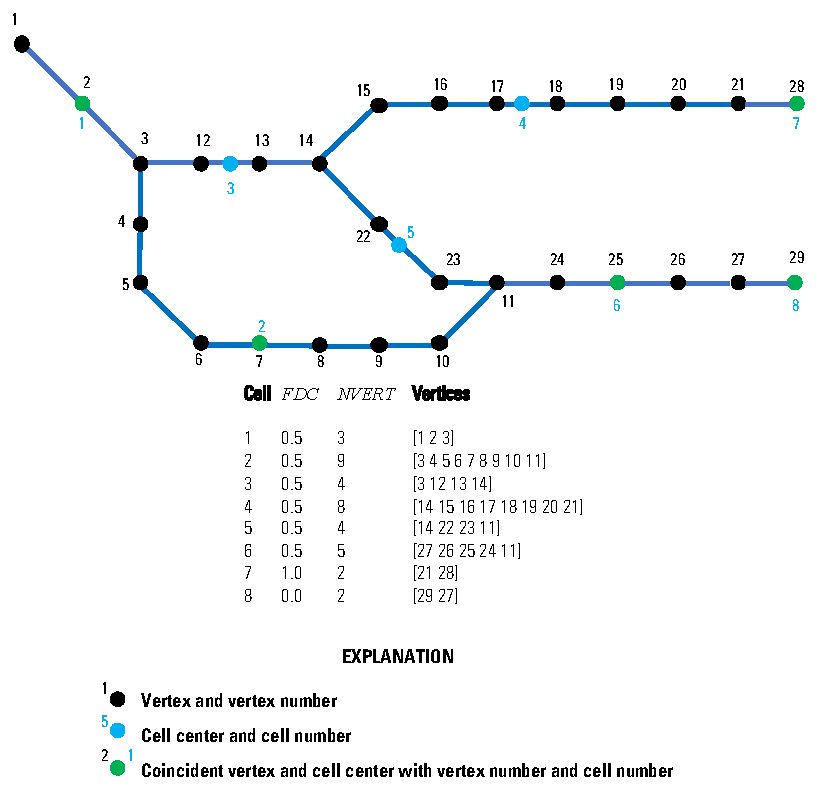
\includegraphics[scale=1.0]{Figures/DISL_example}
	\caption{Schematic diagram showing the vertices and cells defined using the Linear Discretization Package. The list of vertices used to define each cell ordered in either an upstream or downstream direction.  From \cite{modflow6gwf}}
	\label{fig:disl_example}
\end{figure}


\vspace{5mm}
\subsubsection{Structure of Blocks}
\lstinputlisting[style=blockdefinition]{./mf6ivar/tex/lnf-disl-options.dat}
\lstinputlisting[style=blockdefinition]{./mf6ivar/tex/lnf-disl-dimensions.dat}
\lstinputlisting[style=blockdefinition]{./mf6ivar/tex/lnf-disl-griddata.dat}
\lstinputlisting[style=blockdefinition]{./mf6ivar/tex/lnf-disl-vertices.dat}
\lstinputlisting[style=blockdefinition]{./mf6ivar/tex/lnf-disl-cell1d.dat}

\vspace{5mm}
\subsubsection{Explanation of Variables}
\begin{description}
% DO NOT MODIFY THIS FILE DIRECTLY.  IT IS CREATED BY mf6ivar.py 

\item \textbf{Block: OPTIONS}

\begin{description}
\item \texttt{length\_units}---is the length units used for this model.  Values can be ``FEET'', ``METERS'', or ``CENTIMETERS''.  If not specified, the default is ``UNKNOWN''.

\item \texttt{NOGRB}---keyword to deactivate writing of the binary grid file.

\item \texttt{xorigin}---x-position of the origin used for model grid vertices.  This value should be provided in a real-world coordinate system.  A default value of zero is assigned if not specified.  The value for XORIGIN does not affect the model simulation, but it is written to the binary grid file so that postprocessors can locate the grid in space.

\item \texttt{yorigin}---y-position of the origin used for model grid vertices.  This value should be provided in a real-world coordinate system.  If not specified, then a default value equal to zero is used.  The value for YORIGIN does not affect the model simulation, but it is written to the binary grid file so that postprocessors can locate the grid in space.

\item \texttt{angrot}---counter-clockwise rotation angle (in degrees) of the model grid coordinate system relative to a real-world coordinate system.  If not specified, then a default value of 0.0 is assigned.  The value for ANGROT does not affect the model simulation, but it is written to the binary grid file so that postprocessors can locate the grid in space.

\end{description}
\item \textbf{Block: DIMENSIONS}

\begin{description}
\item \texttt{nodes}---is the number of linear cells.

\item \texttt{nvert}---is the total number of (x, y, z) vertex pairs used to characterize the model grid.

\end{description}
\item \textbf{Block: GRIDDATA}

\begin{description}
\item \texttt{idomain}---is an optional array that characterizes the existence status of a cell.  If the IDOMAIN array is not specified, then all model cells exist within the solution.  If the IDOMAIN value for a cell is 0, the cell does not exist in the simulation.  Input and output values will be read and written for the cell, but internal to the program, the cell is excluded from the solution.  If the IDOMAIN value for a cell is 1, the cell exists in the simulation.

\end{description}
\item \textbf{Block: VERTICES}

\begin{description}
\item \texttt{iv}---is the vertex number.  Records in the VERTICES block must be listed in consecutive order from 1 to NVERT.

\item \texttt{xv}---is the x-coordinate for the vertex.

\item \texttt{yv}---is the y-coordinate for the vertex.

\item \texttt{zv}---is the z-coordinate for the vertex.

\end{description}
\item \textbf{Block: CELL1D}

\begin{description}
\item \texttt{icell1d}---is the cell1d number.  Records in the cell1d block must be listed in consecutive order from the first to the last.

\item \texttt{fdc}---is the fractional distance to the cell center. FDC is relative to the first vertex in the ICVERT array. In most cases FDC should be 0.5, which would place the center of the line segment that defines the cell. If the value of FDC is 1, the cell center would located at the last vertex. FDC values of 0 and 1 can be used to place the node at either end of the cell which can be useful for cells with boundary conditions.

\item \texttt{ncvert}---is the number of vertices required to define the cell.  There may be a different number of vertices for each cell.

\item \texttt{icvert}---is an array of integer values containing vertex numbers (in the VERTICES block) used to define the cell.  Vertices must be listed in the order that defines the line representing the cell.  Cells that are connected must share vertices. The bottom elevation of the cell is calculated using the ZV of the first and last vertex point and FDC.

\end{description}


\end{description}

\vspace{5mm}
\subsubsection{Example Input File}
\lstinputlisting[style=inputfile]{./mf6ivar/examples/lnf-disl-example.dat}


\newpage
\subsection{Initial Conditions (IC) Package}
Initial Conditions (IC) Package information is read from the file that is specified by ``IC6'' as the file type.  Only one IC Package can be specified for a GWE model. 

\vspace{5mm}
\subsubsection{Structure of Blocks}
%\lstinputlisting[style=blockdefinition]{./mf6ivar/tex/gwe-ic-options.dat}
\lstinputlisting[style=blockdefinition]{./mf6ivar/tex/gwe-ic-griddata.dat}

\vspace{5mm}
\subsubsection{Explanation of Variables}
\begin{description}
% DO NOT MODIFY THIS FILE DIRECTLY.  IT IS CREATED BY mf6ivar.py 

\item \textbf{Block: OPTIONS}

\begin{description}
\item \texttt{EXPORT\_ARRAY\_ASCII}---keyword that specifies input griddata arrays should be written to layered ascii output files.

\end{description}
\item \textbf{Block: GRIDDATA}

\begin{description}
\item \texttt{strt}---is the initial (starting) temperature---that is, the temperature at the beginning of the GWE Model simulation.  STRT must be specified for all GWE Model simulations. One value is read for every model cell.

\end{description}


\end{description}

\vspace{5mm}
\subsubsection{Example Input File}
\lstinputlisting[style=inputfile]{./mf6ivar/examples/gwe-ic-example.dat}



\newpage
\subsection{Output Control (OC) Option}
Input to the Output Control Option of the Particle Tracking Model is read from the file that is specified as type ``OC6'' in the Name File. If no ``OC6'' file is specified, default output control is used. The Output Control Option determines how and when particle mass budgets are printed to the listing file and/or written to a separate binary output file.  Under the default settings, the particle mass budget is written to the Listing File at the end of every stress period.  The particle mass budget is also written to the list file if the simulation terminates prematurely due to failed convergence.

Output Control data must be specified using words.  The numeric codes supported in earlier MODFLOW versions can no longer be used.

For the PRINT and SAVE options, there is no option to specify individual layers.  Whenever the budget array is printed or saved, all layers are printed or saved.

\vspace{5mm}
\subsubsection{Structure of Blocks}
\vspace{5mm}

\noindent \textit{FOR EACH SIMULATION}
\lstinputlisting[style=blockdefinition]{./mf6ivar/tex/prt-oc-options.dat}
\vspace{5mm}
\noindent \textit{FOR ANY STRESS PERIOD}
\lstinputlisting[style=blockdefinition]{./mf6ivar/tex/prt-oc-period.dat}

\vspace{5mm}
\subsubsection{Explanation of Variables}
\begin{description}
% DO NOT MODIFY THIS FILE DIRECTLY.  IT IS CREATED BY mf6ivar.py 

\item \textbf{Block: OPTIONS}

\begin{description}
\item \texttt{BUDGET}---keyword to specify that record corresponds to the budget.

\item \texttt{FILEOUT}---keyword to specify that an output filename is expected next.

\item \texttt{budgetfile}---name of the output file to write budget information.

\item \texttt{BUDGETCSV}---keyword to specify that record corresponds to the budget CSV.

\item \texttt{budgetcsvfile}---name of the comma-separated value (CSV) output file to write budget summary information.  A budget summary record will be written to this file for each time step of the simulation.

\item \texttt{TRACK}---keyword to specify that record corresponds to a binary track file.

\item \texttt{trackfile}---name of the output file to write tracking information.

\item \texttt{TRACKCSV}---keyword to specify that record corresponds to a CSV track file.

\item \texttt{trackcsvfile}---name of the comma-separated value (CSV) file to write tracking information.

\item \texttt{TRACK\_RELEASE}---keyword to indicate that particle tracking output is to be written when a particle is released

\item \texttt{TRACK\_EXIT}---keyword to indicate that particle tracking output is to be written when a particle exits a cell

\item \texttt{TRACK\_TIMESTEP}---keyword to indicate that particle tracking output is to be written at the end of each time step

\item \texttt{TRACK\_TERMINATE}---keyword to indicate that particle tracking output is to be written when a particle terminates for any reason

\item \texttt{TRACK\_WEAKSINK}---keyword to indicate that particle tracking output is to be written when a particle exits a weak sink (a cell which removes some but not all inflow from adjacent cells)

\item \texttt{TRACK\_USERTIME}---keyword to indicate that particle tracking output is to be written at user-specified times, provided as double precision values to the TRACK\_TIMES or TRACK\_TIMESFILE options

\item \texttt{TRACK\_TIMES}---keyword indicating tracking times will follow

\item \texttt{times}---times to track, relative to the beginning of the simulation.

\item \texttt{TRACK\_TIMESFILE}---keyword indicating tracking times file name will follow

\item \texttt{timesfile}---name of the tracking times file

\end{description}
\item \textbf{Block: PERIOD}

\begin{description}
\item \texttt{iper}---integer value specifying the starting stress period number for which the data specified in the PERIOD block apply.  IPER must be less than or equal to NPER in the TDIS Package and greater than zero.  The IPER value assigned to a stress period block must be greater than the IPER value assigned for the previous PERIOD block.  The information specified in the PERIOD block will continue to apply for all subsequent stress periods, unless the program encounters another PERIOD block.

\item \texttt{SAVE}---keyword to indicate that information will be saved this stress period.

\item \texttt{PRINT}---keyword to indicate that information will be printed this stress period.

\item \texttt{rtype}---type of information to save or print.  Can only be BUDGET.

\item \texttt{ocsetting}---specifies the steps for which the data will be saved.

\begin{lstlisting}[style=blockdefinition]
ALL
FIRST
LAST
FREQUENCY <frequency>
STEPS <steps(<nstp)>
\end{lstlisting}

\item \texttt{ALL}---keyword to indicate save for all time steps in period.

\item \texttt{FIRST}---keyword to indicate save for first step in period. This keyword may be used in conjunction with other keywords to print or save results for multiple time steps.

\item \texttt{LAST}---keyword to indicate save for last step in period. This keyword may be used in conjunction with other keywords to print or save results for multiple time steps.

\item \texttt{frequency}---save at the specified time step frequency. This keyword may be used in conjunction with other keywords to print or save results for multiple time steps.

\item \texttt{steps}---save for each step specified in STEPS. This keyword may be used in conjunction with other keywords to print or save results for multiple time steps.

\end{description}


\end{description}

\vspace{5mm}
\subsubsection{Example Input File}
\lstinputlisting[style=inputfile]{./mf6ivar/examples/prt-oc-example.dat}


